\DAsection[用面板管理 Nginx、进程、数据库与证书]{通过宝塔部署全栈项目}

\begin{frame}{6.1 安装宝塔后的第一件事：加固面板}{面板是高权限管理入口}
  \begin{enumerate}
    \item 从宝塔官网复制当前系统对应的官方安装命令。
    \item 保存安装输出中的面板地址、初始用户名和密码。
    \item 首次登录立即修改强密码、面板端口与安全入口。
    \item 云防火墙限制面板端口来源，优先绑定固定管理 IP。
    \item 开启面板 HTTPS、登录告警与必要的双因素验证。
  \end{enumerate}
  \begin{alertblock}{供应链提醒}
    不使用“破解版 / 纯净版 / 开心版”等第三方修改包，只从官方渠道安装与更新。
  \end{alertblock}
  \DAsource{宝塔官方下载}{https://www.bt.cn/new/download}
\end{frame}

\begin{frame}{6.2 安装基础环境}{Nginx、Node、pnpm、Python 与 MySQL}
  \begin{DAtable}{@{}p{28mm}p{38mm}p{55mm}@{}}
    \toprule
    组件 & 用途 & 选择建议 \\
    \midrule
    Nginx & 80 / 443、静态文件、反向代理 & 必装 \\
    Node.js & 构建前端、运行 Node 后端 / SSR & 安装项目要求的 LTS 版本 \\
    pnpm & Node 依赖与构建 & 通过 Corepack 或官方方式启用 \\
    Python + uv & FastAPI 运行环境 & 与 \DAfile{pyproject.toml} 要求一致 \\
    MySQL & 业务数据 & 本机部署时仅监听本地 / 内网 \\
    \bottomrule
  \end{DAtable}
  \vspace{1mm}
  {\small\textcolor{DARed}{\bfseries 原则：}项目版本来自仓库声明，生产升级要有计划。}
\end{frame}

\begin{frame}[fragile]{6.3 服务器获取代码的推荐方式}{Git Clone + 只读 Deploy Key}
  \begin{lstlisting}[language=bash]
cd /www/wwwroot
git clone git@github.com:your-org/customer-service.git
cd customer-service

git switch main
git pull --ff-only
git rev-parse --short HEAD
  \end{lstlisting}
  \begin{itemize}
    \item 服务器只负责部署时，Deploy Key 尽量设为只读。
    \item 记录当前 Commit ID，后续更新与回滚都以它为坐标。
    \item 不在服务器直接改业务代码，否则 Git 历史与线上状态会分叉。
  \end{itemize}
\end{frame}

\begin{frame}[fragile]{6.4 构建 Node 前端}{依赖锁定，API 地址使用生产配置}
  \begin{lstlisting}[language=bash]
cd /www/wwwroot/customer-service/frontend

corepack enable
pnpm install --frozen-lockfile
pnpm build

ls -la dist
  \end{lstlisting}
  \begin{itemize}
    \item Vite 常见输出目录是 \DAfile{dist/}；其他框架以项目配置为准。
    \item 推荐前端请求相对路径 \DAfile{/api}，由 Nginx 转发到后端。
    \item 构建时环境变量会写入静态文件，修改后必须重新构建。
  \end{itemize}
\end{frame}

\begin{frame}{6.5 创建静态站点}{网站根目录指向构建产物}
  \begin{enumerate}
    \item 宝塔左侧进入“网站”，添加站点并填写域名。
    \item 站点类型选择纯静态；根目录指向前端 \DAfile{dist/}。
    \item 确认运行用户对目录有读取权限。
    \item 暂时可用 HTTP 验证首页资源是否正确加载。
    \item 浏览器 F12 检查 HTML、JS、CSS 是否全部 200。
  \end{enumerate}
  \DAtagline{网站根目录}{只指向 \DAfile{dist/} 等生产构建产物}
  \DAsource{宝塔官方文档 · 添加站点}{https://docs.bt.cn/user-guide/site/php/create-web}
\end{frame}

\begin{frame}[fragile]{6.6 SPA 刷新 404 怎么修}{让未知前端路由回到 index.html}
  \begin{lstlisting}[language=bash]
location / {
    try_files $uri $uri/ /index.html;
}
  \end{lstlisting}
  \begin{itemize}
    \item React Router / Vue Router 的 History 模式由浏览器管理路由。
    \item 用户直接访问 \DAfile{/chat/123} 时，Nginx 找不到同名文件会返回 404。
    \item \DAcmd{try\_files} 让前端路由接管；\DAfile{/api} 保持独立代理规则。
  \end{itemize}
\end{frame}

\begin{frame}[fragile]{6.7 准备 FastAPI 生产环境}{服务器按锁文件创建独立虚拟环境}
  \begin{lstlisting}[language=bash]
cd /www/wwwroot/customer-service/backend

uv sync --locked --no-dev
uv run python -m pytest

uv run fastapi run app/main.py \
  --host 127.0.0.1 --port 8000 --proxy-headers
  \end{lstlisting}
  \begin{itemize}
    \item 先前台启动并用 \DAcmd{curl http://127.0.0.1:8000/health} 验证。
    \item 监听 \DAfile{127.0.0.1}，业务端口只允许本机 Nginx 访问。
    \item 确认无误后再交给宝塔项目管理 / 应用管理器守护。
  \end{itemize}
\end{frame}

\begin{frame}{6.8 FastAPI 进程守护}{SSH 断开后仍运行，异常后能重启}
  \begin{DAtable*}{@{}p{31mm}p{84mm}@{}}
    \toprule
    配置项 & 示例 \\
    \midrule
    项目目录 & \DAfile{/www/wwwroot/customer-service/backend} \\
    Python 环境 & 项目 \DAfile{.venv} 中的 Python / FastAPI \\
    启动命令 & 使用上一页命令，监听 \DAfile{127.0.0.1:8000} \\
    运行用户 & 非 root，确保能读代码与写日志 / 上传目录 \\
    环境变量 & 通过面板项目配置或受控 Env 文件注入 \\
    重启策略 & 开机启动、异常退出自动重启 \\
    \bottomrule
  \end{DAtable*}
  \DAtagline*{版本差异}{不同宝塔版本入口可能显示为 Python 项目、应用管理器或进程守护}
\end{frame}

\begin{frame}[fragile]{6.9 Nginx 把 /api 转给 FastAPI}{同域部署减少 CORS 与 Cookie 问题}
  \begin{lstlisting}[language=bash]
location /api/ {
    proxy_pass http://127.0.0.1:8000/;
    proxy_set_header Host $host;
    proxy_set_header X-Real-IP $remote_addr;
    proxy_set_header X-Forwarded-For $proxy_add_x_forwarded_for;
    proxy_set_header X-Forwarded-Proto $scheme;
}
  \end{lstlisting}
  \begin{itemize}
    \item 访问 \DAfile{https://app.example.com/api/health}，Nginx 转给 FastAPI。
    \item 注意 \DAcmd{proxy\_pass} 末尾斜杠会影响路径改写，必须现场验证真实路由。
    \item 后端启用 Proxy Headers 后，才能正确感知外部协议与客户端信息。
  \end{itemize}
  \DAsource{NGINX Docs · Reverse Proxy}{https://docs.nginx.com/nginx/admin-guide/web-server/reverse-proxy/}
\end{frame}

\begin{frame}{6.10 宝塔反向代理界面}{面板字段与 Nginx 配置一一对应}
  \begin{columns}[T]
    \begin{column}{0.42\textwidth}
      \begin{itemize}
        \item 代理名称：\DAfile{fastapi-api}
        \item 代理目录：\DAfile{/api/}
        \item 目标 URL：\DAfile{http://127.0.0.1:8000}
        \item 发送域名：通常使用 \DAfile{\$host}
        \item API 默认关闭缓存
      \end{itemize}
    \end{column}
    \begin{column}{0.54\textwidth}
      \centering
      \DAframed{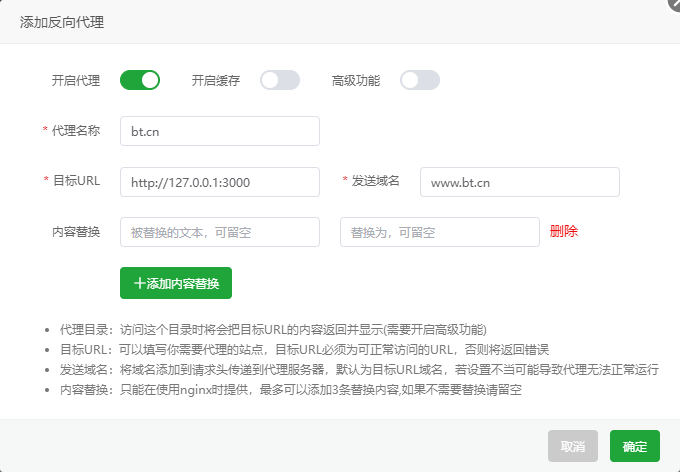
\includegraphics[width=68mm]{assets/official/bt-add-reverse-proxy.png}}
    \end{column}
  \end{columns}
  \DAsource{宝塔官方文档 · 反向代理}{https://docs.bt.cn/user-guide/site/php/site-config/reverse-proxy}
\end{frame}

\begin{frame}{6.11 前后端联调的验证顺序}{后端、Nginx、浏览器逐层检查}
  \begin{enumerate}
    \item \DAcmd{curl http://127.0.0.1:8000/health}：后端进程是否正常。
    \item \DAcmd{curl -i http://127.0.0.1/api/health}：Nginx 反代是否正常。
    \item 浏览器打开域名：前端静态资源是否正常。
    \item F12 Network 查看 \DAfile{/api/...} 请求、状态码、响应体。
    \item 后端日志确认同一请求是否到达、耗时与错误。
  \end{enumerate}
  \DAtagline{定位法}{在哪一层第一次失败，问题就位于该层或它的下一跳}
\end{frame}

\begin{frame}[fragile]{6.12 Node.js 后端部署}{pnpm 构建 + PM2 / 宝塔 Node 项目守护}
  \begin{lstlisting}[language=bash]
cd /www/wwwroot/customer-service/server

corepack enable
pnpm install --frozen-lockfile
pnpm build
pnpm start
  \end{lstlisting}
  \begin{itemize}
    \item Express / NestJS 等后端通常监听 \DAfile{127.0.0.1:3000}。
    \item 宝塔 Node 项目管理默认可使用 PM2 做守护与自动重启。
    \item Nginx 的目标 URL 改为 \DAfile{http://127.0.0.1:3000}，其他思路相同。
  \end{itemize}
  \DAsource{宝塔官方文档 · Node.js PM2 部署}{https://docs.bt.cn/practical-tutorials/nodejs-pm2-deployment}
\end{frame}

\begin{frame}{6.13 宝塔 Node 项目配置示意}{项目路径、启动命令、端口和运行用户}
  \begin{DAfigrow}
    \DAfigbox*{25mm}{assets/official/bt-node-project.png}{添加 Node 项目 · 宝塔官方}\hfill
    \DAfigbox*{25mm}{assets/official/bt-node-port.png}{配置启动端口 · 宝塔官方}
  \end{DAfigrow}
  \DAtagline{pnpm}{找不到命令时先确认 Node 版本与 PATH，避免重复安装}
  \DAsource{宝塔官方文档 · Next.js 部署}{https://docs.bt.cn/practical-tutorials/nextjs-deployment}
\end{frame}

\begin{frame}{6.14 环境变量如何放到服务器}{仓库保存变量名，服务器保存真实值}
  \begin{DAtable}{@{}p{35mm}p{82mm}@{}}
    \toprule
    类型 & 处理方式 \\
    \midrule
    前端公开配置 & 构建时注入；默认视为用户可见，不放 Secret \\
    后端普通配置 & 项目环境变量或权限受控的 Env 文件 \\
    数据库密码 / API Key & 最小权限、定期轮换、日志脱敏 \\
    JWT Secret & 使用足够随机值，变更会影响现有 Token \\
    上传目录 & 独立持久目录，权限给运行用户并纳入备份 \\
    \bottomrule
  \end{DAtable}
  \DAtagline{权限}{Env 文件只允许部署用户 / 运行用户读取，避免通过静态站点暴露}
\end{frame}

\begin{frame}[fragile]{6.15 宝塔手工更新顺序}{构建、备份、切换、验证}
  \begin{lstlisting}[language=bash]
cd /www/wwwroot/customer-service
git fetch origin
git switch main
git pull --ff-only

cd frontend
pnpm install --frozen-lockfile
pnpm build

cd ../backend
uv sync --locked --no-dev
# run migrations, then restart backend in panel
  \end{lstlisting}
  \begin{itemize}
    \item 更新前记录旧 Commit ID、备份数据库与上传文件。
    \item 依赖、迁移、重启、健康检查必须按 SOP 执行。
    \item 不在用户高峰期第一次尝试未知升级步骤。
  \end{itemize}
\end{frame}

\begin{frame}{6.16 宝塔部署最常见的 502}{Nginx 找不到或无法连接上游服务}
  \begin{columns}[T]
    \begin{column}{0.48\textwidth}
      \begin{itemize}
        \item 后端进程没有启动或持续崩溃。
        \item 代理目标端口写错。
        \item 应用只监听容器 / 其他网卡。
        \item 权限、依赖或环境变量导致启动失败。
        \item Nginx 配置未重载或语法错误。
      \end{itemize}
    \end{column}
    \begin{column}{0.48\textwidth}
      \begin{block}{排查证据}
        \begin{itemize}
          \item 项目状态与启动日志
          \item \DAcmd{ss -lntp}
          \item 本机 \DAcmd{curl} 上游端口
          \item Nginx error log
          \item 应用 error / access log
        \end{itemize}
      \end{block}
    \end{column}
  \end{columns}
  \DAtagline{顺序}{先验证上游进程，再检查 Nginx 配置与日志}
\end{frame}
